\pc{1}{17/1}

\question Show how any non-deterministic finite automaton can be represented with a
deterministic finite automaton.
\begin{solution}
    The strategy here is to contrust a determinstic finite automaton where
    each state represents a set of states possible with the input
    in the non-determinstic finite automaton.
\end{solution}

\question 
\begin{parts}
    \part Construct a 3-state non-deterministic finite automaton over a binary alphabet,
    $\{0, 1\}$,
    that accepts precisely the words that have $1$ in the position before the last.
    \begin{solution}
        \begin{center}
            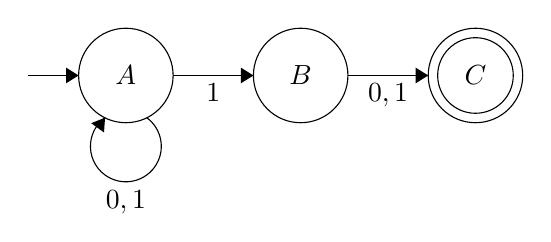
\begin{tikzpicture}[scale=0.2]
                \tikzstyle{every node}+=[inner sep=0pt]
                \draw [black] (11.8,-23.9) circle (3);
                \draw (11.8,-23.9) node {$A$};
                \draw [black] (22.9,-23.9) circle (3);
                \draw (22.9,-23.9) node {$B$};
                \draw [black] (34,-23.9) circle (3);
                \draw (34,-23.9) node {$C$};
                \draw [black] (34,-23.9) circle (2.4);
                \draw [black] (5.6,-23.9) -- (8.8,-23.9);
                \fill [black] (8.8,-23.9) -- (8,-23.4) -- (8,-24.4);
                \draw [black] (13.123,-26.58) arc (54:-234:2.25);
                \draw (11.8,-31.15) node [below] {$0,1$};
                \fill [black] (10.48,-26.58) -- (9.6,-26.93) -- (10.41,-27.52);
                \draw [black] (14.8,-23.9) -- (19.9,-23.9);
                \fill [black] (19.9,-23.9) -- (19.1,-23.4) -- (19.1,-24.4);
                \draw (17.35,-24.4) node [below] {$1$};
                \draw [black] (25.9,-23.9) -- (31,-23.9);
                \fill [black] (31,-23.9) -- (30.2,-23.4) -- (30.2,-24.4);
                \draw (28.45,-24.4) node [below] {$0,1$};
            \end{tikzpicture}
        \end{center}
    \end{solution}

    \part Convert this to a deterministic finite automaton.
    \begin{solution}
        \begin{center}
            \footnotesize
            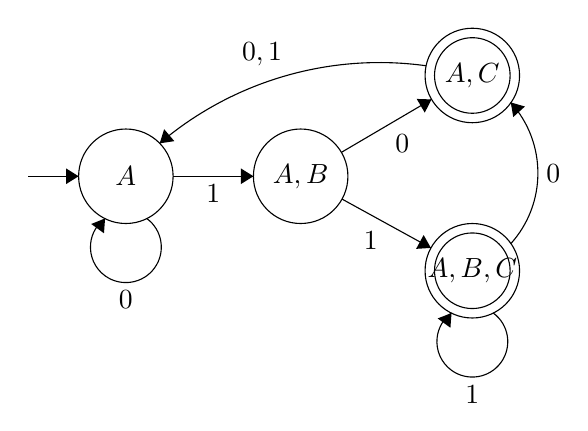
\begin{tikzpicture}[scale=0.2]
                \tikzstyle{every node}+=[inner sep=0pt]
                \draw [black] (11.8,-23.9) circle (3);
                \draw (11.8,-23.9) node {$A$};
                \draw [black] (22.9,-23.9) circle (3);
                \draw (22.9,-23.9) node {$A,B$};
                \draw [black] (33.8,-17.5) circle (3);
                \draw (33.8,-17.5) node {$A,C$};
                \draw [black] (33.8,-17.5) circle (2.4);
                \draw [black] (33.8,-29.9) circle (3);
                \draw (33.8,-29.9) node {$A,B,C$};
                \draw [black] (33.8,-29.9) circle (2.4);
                \draw [black] (5.6,-23.9) -- (8.8,-23.9);
                \fill [black] (8.8,-23.9) -- (8,-23.4) -- (8,-24.4);
                \draw [black] (13.123,-26.58) arc (54:-234:2.25);
                \draw (11.8,-31.15) node [below] {$0$};
                \fill [black] (10.48,-26.58) -- (9.6,-26.93) -- (10.41,-27.52);
                \draw [black] (36.235,-19.209) arc (42.11563:-42.11563:6.697);
                \fill [black] (36.24,-19.21) -- (36.4,-20.14) -- (37.14,-19.47);
                \draw (38.46,-23.7) node [right] {$0$};
                \draw [black] (35.123,-32.58) arc (54:-234:2.25);
                \draw (33.8,-37.15) node [below] {$1$};
                \fill [black] (32.48,-32.58) -- (31.6,-32.93) -- (32.41,-33.52);
                \draw [black] (25.53,-25.35) -- (31.17,-28.45);
                \fill [black] (31.17,-28.45) -- (30.71,-27.63) -- (30.23,-28.51);
                \draw (27.35,-27.4) node [below] {$1$};
                \draw [black] (25.49,-22.38) -- (31.21,-19.02);
                \fill [black] (31.21,-19.02) -- (30.27,-18.99) -- (30.78,-19.86);
                \draw (29.35,-21.2) node [below] {$0$};
                \draw [black] (14.8,-23.9) -- (19.9,-23.9);
                \fill [black] (19.9,-23.9) -- (19.1,-23.4) -- (19.1,-24.4);
                \draw (17.35,-24.4) node [below] {$1$};
                \draw [black] (13.945,-21.806) arc (130.31957:82.12082:21.579);
                \fill [black] (13.95,-21.81) -- (14.88,-21.67) -- (14.23,-20.91);
                \draw (20.45,-16.95) node [above] {$0,1$};
            \end{tikzpicture}
        \end{center}    
    \end{solution}
\end{parts}

\question Let $A$ and $B$ be two B\"uchi automata.
\begin{parts}
    \part Construct an automaton that implements the union of $A$ and $B$.
    \begin{solution}
        Let 
        $A_1 = (\Sigma, Q, Q_0, F_1, \delta_1)$
        and 
        $A_2 = (\Sigma, P, P_0, F_2, \delta_2)$
        be our two B\"uchi automata.
        Then
        \[
            A_1 \cup A_2 = 
            (\Sigma, Q \cup P, Q_0 \cup P_0, F_1 \cup F_2, \delta_1 \cup \delta_2)
        \]
        implements our union.
    \end{solution}

    \part Construct an automaton that implements the intersection of $A$ and $B$.
    \begin{solution}
        Let $A_1$ and $A_2$ be as in the previous example.
        Then
        \[
            A_1 \cap A_2
            = (\Sigma, Q \times P, Q_0 \times P_0, F_1 \times F_2, \delta)
        \]
        where $\delta((q,p),a) = (\delta(p,a), \delta(q,a))$
        with $p,q \in Q\times P$ and $a \in \Sigma$.
        This automaton implements our intersection.
    \end{solution}
\end{parts}
